\chapter{序論}

\section{背景}

VR（Virtual Reality）ゲームでは，仮想空間への没入感や，炎やビームなどの攻撃エフェクトによる迫力ある演出が，ゲーム体験を構成する重要な要素となっている．一方，画面内で手前の物体が奥の対象物を隠す遮蔽は，対象物の位置や形状を把握しにくくする問題を引き起こす．この問題に対して，対象物の視認性を確保するため，遮蔽物を半透明にする手法や，対象物の輪郭を強調する手法などが用いられている．

\section{課題}

VRゲームの攻撃エフェクトは迫力や臨場感を生み出す一方で，プレイヤーの視点と攻撃対象との間に表示されることで，対象物を隠してしまう場合がある．特に，プレイヤー自身の口から炎などを放出するブレス攻撃では，攻撃エフェクトによる遮蔽が対象物の追従や攻撃の正確性に影響する可能性がある．

\begin{figure}[htbp]
  \centering
  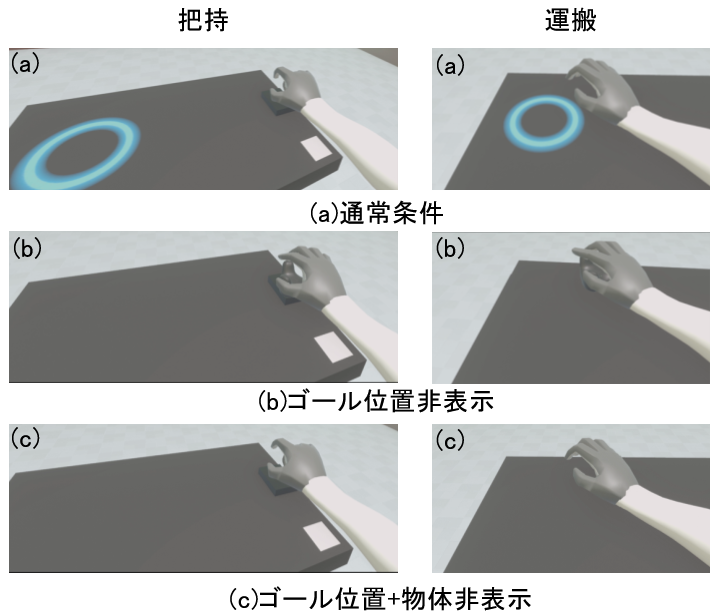
\includegraphics[width=0.5\linewidth]{fig/act5.png}
  \caption{エフェクトによって対象が見えていない画像予定}
  \label{fig:1}
\end{figure}


しかし，視認性を高めるためにエフェクト全体を半透明にすると，攻撃の力強さや視覚的な迫力が損なわれる課題がある.

\section{目的}
本研究では,視認性とゲーム体験を両立できる攻撃エフェクトの表示方法を調査する。
